\documentclass[aspectratio=169]{beamer}

% ---------- Theme & Colors ----------
\usetheme{Madrid}
\usecolortheme{whale}
\definecolor{darkblue}{RGB}{37,47,130}
\definecolor{midblue}{RGB}{70,90,200}
\definecolor{lightblue}{RGB}{180,200,255}
\definecolor{alertred}{RGB}{200,50,50}
\definecolor{successgreen}{RGB}{30,160,80}

\setbeamercolor{frametitle}{bg=darkblue, fg=white}
\setbeamercolor{title}{bg=darkblue, fg=white}
\setbeamercolor{section in toc}{fg=darkblue}
\setbeamercolor{block title}{bg=darkblue, fg=white}
\setbeamercolor{block body}{bg=lightblue!30}
\setbeamercolor{alerted text}{fg=alertred}
\setbeamercolor{structure}{fg=darkblue}

\setbeamertemplate{navigation symbols}{} % Remove navigation symbols

% ---------- Packages ----------
\usepackage{amsmath, amssymb, amsthm}
\usepackage{tikz}
\usepackage{pgfplots}
\pgfplotsset{compat=1.18}
\usetikzlibrary{arrows.meta, positioning, shapes.geometric, decorations.pathreplacing,
                patterns, calc, backgrounds, fit}
\usepackage{booktabs}
\usepackage{xcolor}
\usepackage{mathtools}
\usepackage{bm}
\usepackage{graphicx}


% ---------- Custom Commands ----------
\newcommand{\E}{\mathbb{E}}
\newcommand{\Var}{\mathrm{Var}}
\newcommand{\R}{\mathbb{R}}
\newcommand{\calD}{\mathcal{D}}
\newcommand{\calX}{\mathcal{X}}
\newcommand{\calY}{\mathcal{Y}}
\newcommand{\calC}{\mathcal{C}}
\newcommand{\btheta}{\bm{\theta}}


% Title page information
\title[UQ in Data Science]{Uncertainty Quantification}
\author{Lecturer Name}
\date{\today}

\begin{document}

% Slide 1: Title
\begin{frame}
    \titlepage
\end{frame}

% Summary Slide
\begin{frame}{Summary}
  \begin{itemize}
    \item \textbf{UQ goal:} quantify predictive uncertainty to support safe decisions.
    \item \textbf{Key concepts:} prediction vs.\ confidence vs.\ calibration.
    \item \textbf{Diagnostics:} reliability diagrams, Brier score (Murphy decomposition), NLL.
    \item \textbf{Decision tools:} uncertainty thresholding, coverage vs.\ accuracy trade-offs.
    \item \textbf{Regression UQ:} interval coverage (PICP) and width (MPIW).
  \end{itemize}
\end{frame}

% Outline (shown at the start of each section)
\AtBeginSection[]
{
    \begin{frame}{Outline}
        \tableofcontents[currentsection]
    \end{frame}
}

% Section: Introduction
\section{Introduction}

\begin{frame}[plain]
    \centering
    \vfill
    {\usebeamerfont{section title}Introduction \par}
    \vfill
  \end{frame}


% Slide 2: Overview
\begin{frame}{Motivation}
    \framesubtitle{Why are we here?}
    \begin{columns}[T,onlytextwidth]
        \begin{column}{0.55\textwidth}
            \begin{itemize}
        \item \textbf{The Data Science Standard:} We often optimize models to minimize average loss (e.g., MSE, Cross-Entropy) and maximize point-prediction accuracy.
        \vspace{0.3cm}
        \item \textbf{The Real-World Problem:} Models are deployed in environments different from their training distributions.
        \vspace{0.3cm}
        \item \textbf{The Shift in Paradigm:} From asking \textit{"What is the most likely outcome?"} to \textit{"What is the distribution of possible outcomes, and when should the model say 'I don't know'?"}
            \end{itemize}
        \end{column}
        \begin{column}{0.45\textwidth}
            \centering
            % Upload an image file named motivation-image.(pdf|png|jpg) into the project.
            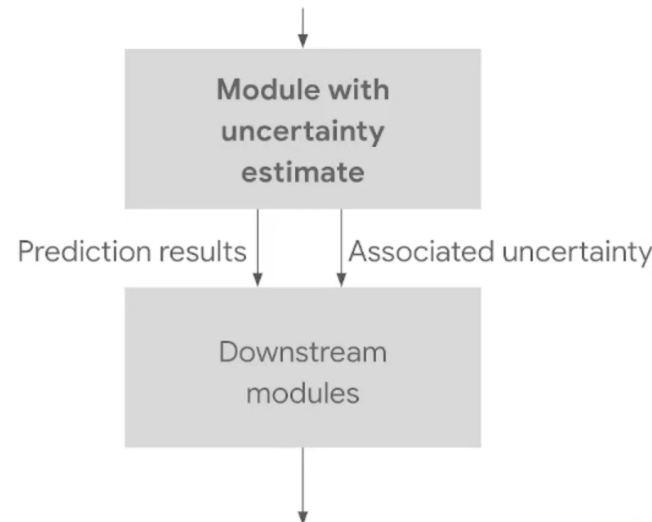
\includegraphics[width=\linewidth]{images/intro.png}
        \end{column}
    \end{columns}
\end{frame}

% Slide 3: Why UQ Matters
\begin{frame}{Why Uncertainty Quantification Matters}
    \begin{itemize}
        \item \textbf{Decision Making:} Moving beyond predictive modeling to prescriptive analytics. Optimizing interventions requires understanding risk profiles and worst-case bounds.
        \vspace{0.2cm}
        \item \textbf{Safety-Critical AI:} 
        \begin{itemize}
            \item \textit{Medicine:} When should an AI system defer a diagnosis to a human clinician?
            \item \textit{Autonomous Systems:} How does a self-driving car react to out-of-distribution (OOD) sensor data?
        \end{itemize}
        \vspace{0.2cm}
        \item \textbf{Model Reliability vs. Accuracy:} A highly accurate model on a static test set can be catastrophically brittle in production. Reliability demands knowing the boundaries of model competence.
    \end{itemize}
\end{frame}

% Slide 3a: Use case 1
\begin{frame}{Use Case: Clinical Diagnosis}
    \begin{columns}[T,onlytextwidth]
        \begin{column}{0.4\textwidth}
            \begin{itemize}
                \item \textbf{Why UQ:} Calibrated probabilities support thresholding, escalation, and \textit{defer-to-human} decisions.
            \end{itemize}
        \end{column}
        \begin{column}{0.6\textwidth}
            \centering
            % Upload an image file named clinical-risk.(pdf|png|jpg) into the project.
            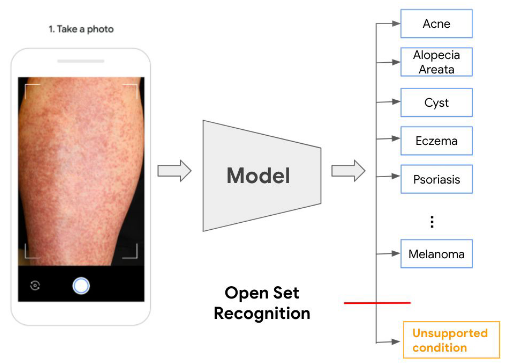
\includegraphics[width=\linewidth]{images/intro2.png}
        \end{column}
    \end{columns}
    \scriptsize

    https://blog.google/technology/health/ai-dermatology-preview-io-2021/
\end{frame}

% Slide 3b: Use case 2
\begin{frame}{Use Case: Active Learning}
\begin{columns}[T,onlytextwidth]
    \begin{column}{0.55\textwidth}
        \begin{itemize}
            \item \textbf{Goal:} Minimize labeling cost by choosing \emph{which} data points to label next.
            \vspace{0.2cm}
            \item \textbf{UQ as the selection signal:} Prefer points with high \emph{epistemic} uncertainty (model doesn't know), not just noisy observations.
            \vspace{0.2cm}
            \item \textbf{Typical loop:}
            \begin{enumerate}
                \item Train on labeled set $\mathcal{D}_L$
                \item Score pool $\mathcal{D}_U$ using an acquisition function $a(x)$
                \item Label top-$k$ points, update $\mathcal{D}_L$, repeat
            \end{enumerate}
            \vspace{0.2cm}
        \end{itemize}
    \end{column}
    \begin{column}{0.45\textwidth}
        \centering
        % Upload an image file named active-learning.(pdf|png|jpg) into the project.
        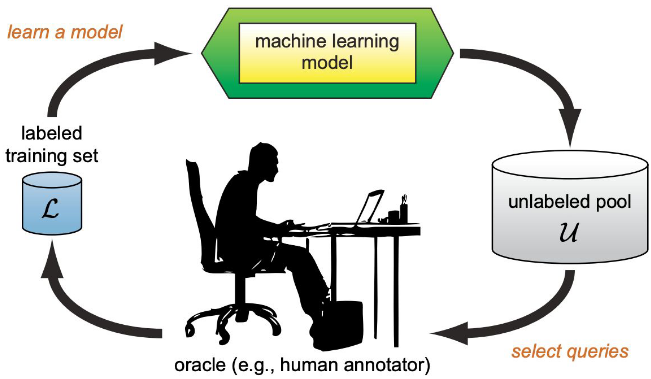
\includegraphics[width=\linewidth]{images/intro3.png}
    \end{column}
\end{columns}

\scriptsize

    https://www.gatsby.ucl.ac.uk/~balaji/balaji-uncertainty-talk-cifar-dlrl.pdf
\end{frame}



% Slide 4: Prediction, Confidence, Calibration
\begin{frame}{Prediction vs. Confidence vs. Calibration}
    \begin{block}{The Miscalibration Problem}
        Modern deep neural networks are highly accurate but notoriously \textbf{overconfident}. A softmax output of $0.99$ does \textit{not} mean a 99\% probability of correctness.
    \end{block}
    
    \begin{itemize}
        \item \textbf{Prediction:} The model's point estimate $\hat{y}$ (e.g., class label or mean regression value).
        \item \textbf{Confidence:} The model's internal score or probability estimate for its prediction.
        \item \textbf{Calibration:} The alignment between confidence and empirical accuracy. If a model predicts an event with 80\% confidence, that event should occur 80\% of the time.
    \end{itemize}
    
    \vspace{0.2cm}
    \textit{Goal of UQ: Achieve perfect calibration without sacrificing predictive power.}
\end{frame}

% Slide 4a: Example --- Prediction
\begin{frame}{Example: Prediction (Point Estimate)}
    \begin{itemize}
        \item \textbf{Classification:} $\hat{y}=\arg\max_k p_\theta(y=k\mid x)$ is the predicted class label.

        \item \textbf{Regression:} $\hat{y}=\mathbb{E}[Y\mid X=x]$ (often approximated by the network output) is the predicted mean.
 
        \item \textbf{Key point:} Prediction alone says \emph{what} the model thinks will happen, but not \emph{how sure} it is.
    \end{itemize}


    \centering
    % Upload an image file named prediction-example.(pdf|png|jpg) into the project.
    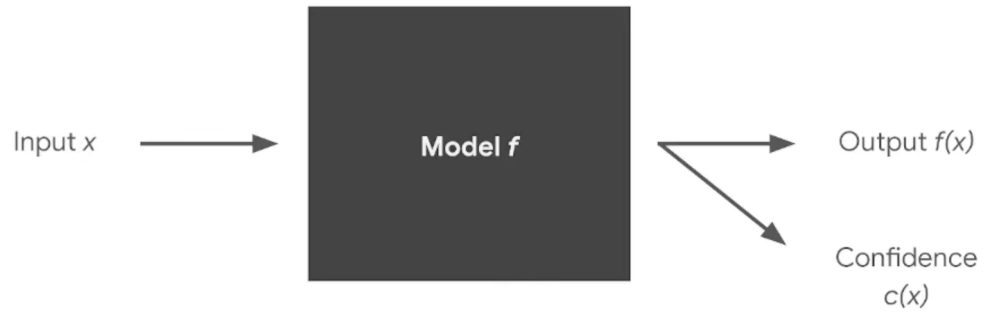
\includegraphics[width=0.75\linewidth]{images/uq_ex1.png}


\end{frame}

% Slide 4b: Example --- Confidence
\begin{frame}{Example: Confidence}
    \begin{itemize}
        \item \textbf{Example:} A classifier outputs softmax scores
        \[
            p_\theta(y\mid x) = (0.60,\,0.25,\,0.15)
        \]
        and predicts class 1 with \textbf{confidence} $0.60$.

        \item \textbf{Important:} Confidence is a \emph{model-internal} number; it can be high even when wrong (especially OOD).

    \end{itemize}


    \centering
    % Upload an image file named confidence-example.(pdf|png|jpg) into the project.
    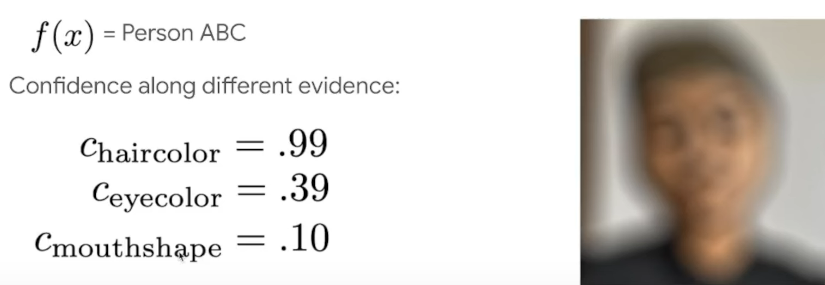
\includegraphics[width=0.75\linewidth]{images/uq_ex2.png}


\end{frame}



% Slide 4b (image only): Confidence figure
\begin{frame}{Example: Confidence in image reconstruction}
    \centering
    % Upload an image file named confidence-only.(pdf|png|jpg) into the project.
    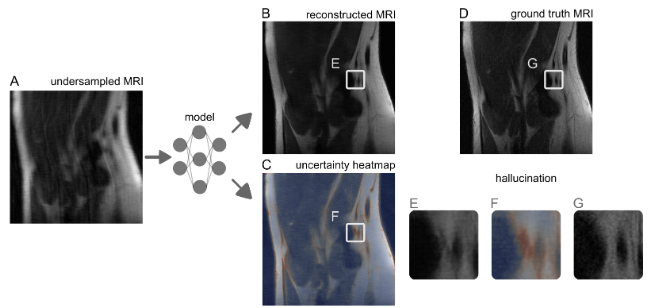
\includegraphics[width=0.9\linewidth,height=\textheight,keepaspectratio]{images/uq_ex3.png}

    \scriptsize

    A. N. Angelopoulos et al., “Image-to-image regression with distribution-free uncertainty quantification and applications in imaging,” PMLR, https://proceedings.mlr.press/v162/angelopoulos22a.html . 
\end{frame}

% Slide 4b (image only): Confidence figure
\begin{frame}{Example: Confidence in regression}
    \centering
    % Upload an image file named confidence-only.(pdf|png|jpg) into the project.
    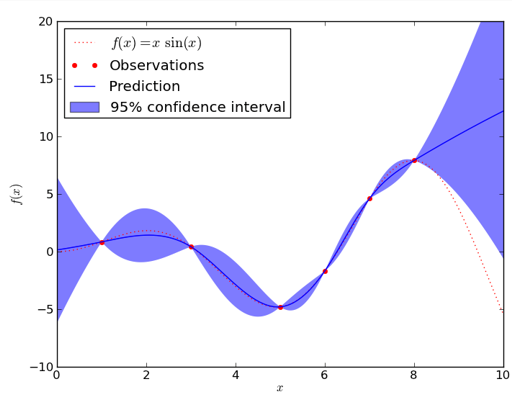
\includegraphics[width=0.6\linewidth]{images/uq_ex4.png}
\end{frame}


% Slide 4b: Example --- Confidence (classification)
\begin{frame}{Example: Confidence in classification}
    \begin{columns}[T,onlytextwidth]
        \begin{column}{0.55\textwidth}
            \begin{itemize}
                \item \textbf{Example:} A classifier outputs softmax probabilities
                \[
                    p_\theta(y\mid x) = (0.60,0.40)
                \]
                and predicts class 1 with confidence $0.60$.
                \vspace{0.2cm}
                \item \textbf{Note:} High confidence does not necessarily mean correctness (especially under distribution shift / OOD).
            \end{itemize}
        \end{column}
        \begin{column}{0.45\textwidth}
            \centering
            % TikZ sketch: softmax confidence over classes
            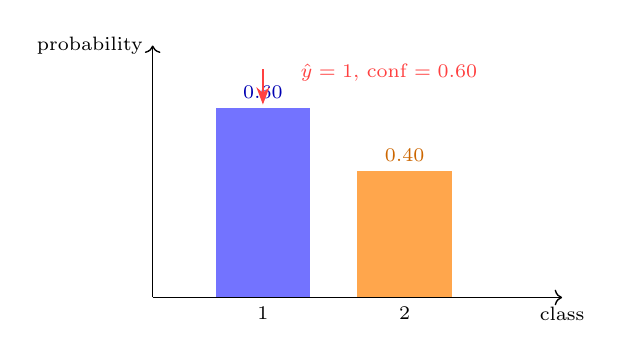
\begin{tikzpicture}[x=1cm,y=1cm]
                % Axis
                \draw[->,line width=0.5pt] (0,0) -- (5.2,0) node[below] {\scriptsize class};
                \draw[->,line width=0.5pt] (0,0) -- (0,3.2) node[left] {\scriptsize probability};

                % Bars
                \fill[blue!55]   (0.8,0) rectangle (2.0,2.4);
                \fill[orange!70] (2.6,0) rectangle (3.8,1.6);


                % Labels under bars
                \node[below] at (1.4,0) {\scriptsize $1$};
                \node[below] at (3.2,0) {\scriptsize $2$};


                % Probability labels
                \node[above,blue!70!black] at (1.4,2.4) {\scriptsize $0.60$};
                \node[above,orange!80!black] at (3.2,1.6) {\scriptsize $0.40$};


                % Arrow to predicted class
                \draw[-{Stealth[length=2.2mm]},red!75,line width=0.7pt] (1.4,2.9) -- (1.4,2.45);
                \node[red!75] at (3.0,2.85) {\scriptsize $\hat{y}=1$, conf $=0.60$};
            \end{tikzpicture}
        \end{column}
    \end{columns}
\end{frame}

% Slide 4c: Example --- Calibration
\begin{frame}{Example: Calibration (Confidence vs. Accuracy)}
    \begin{columns}[T,onlytextwidth]
        \begin{column}{0.52\textwidth}
            \begin{itemize}
                \item \textbf{Definition:} A model is \textbf{well-calibrated} if, among predictions made with confidence $c$, the empirical accuracy is also $c$.
                \vspace{0.2cm}
                              \item \textbf{Concrete example:} Of all predictions made at 0.80 confidence, roughly 80\% should be correct.
                \vspace{0.2cm}
                \item \textbf{Diagnostic:} Reliability diagram.
            \end{itemize}
        \end{column}
        \begin{column}{0.48\textwidth}
            \centering
            \begin{tikzpicture}[x=4.8cm,y=4.8cm]
                % Axes
                \draw[->,line width=0.5pt] (0,0) -- (1.05,0) node[below] {\scriptsize Confidence};
                \draw[->,line width=0.5pt] (0,0) -- (0,1.05) node[left] {\scriptsize Accuracy};

                % Perfect calibration line
                \draw[black!60,dashed,line width=0.6pt] (0,0) -- (1,1);
                \node[black!60,anchor=south east] at (1,1) {\scriptsize $y=x$};

                % Example (slightly miscalibrated) curve
                \draw[blue!70,line width=0.8pt]
                    (0.05,0.10)
                    .. controls (0.25,0.22) and (0.35,0.35) .. (0.50,0.48)
                    .. controls (0.65,0.63) and (0.80,0.72) .. (0.95,0.85);

                % A few bin markers
                \foreach \x/\y in {0.2/0.18,0.4/0.36,0.6/0.58,0.8/0.73} {
                    \fill[blue!70] (\x,\y) circle (0.012);
                }
            \end{tikzpicture}

            \vspace{0.15cm}
            \scriptsize Reliability diagram: compare the curve to the dashed $y=x$ line.
        \end{column}
    \end{columns}


\end{frame}


% ================================================================
\section{Taxonomy of Uncertainty}
% ================================================================

\begin{frame}[plain]
    \centering
    \vfill
    {\usebeamerfont{section title}Taxonomy of Uncertainty \par}
    \vfill
  \end{frame}


% =============================================================
\begin{frame}{The Bayesian Predictive Distribution}

  \begin{block}{Classical (point-estimate) perspective}
    Pick the single ``best'' parameters $\hat\btheta$ (e.g.\ via MLE/MAP), then predict
    $p(y \mid x, \hat\btheta)$.
    \par\smallskip
    \textbf{Problem:} We ignore all other plausible parameter values — ignoring parameter
    uncertainty entirely.
  \end{block}

  \vspace{0.4em}
  \begin{alertblock}{Bayesian predictive distribution}
    \[
      \underbrace{p(y \mid x, \calD)}_{\text{full predictive}}
      \;=\;
      \int
        \underbrace{p(y \mid x, \btheta)}_{\text{likelihood}}
        \;\cdot\;
        \underbrace{p(\btheta \mid \calD)}_{\text{posterior}}
      \; d\btheta
      \;=\;
      \E_{p(\btheta|\calD)}\!\left[p(y\mid x,\btheta)\right]
    \]
  \end{alertblock}

  \vspace{0.3em}
  \textbf{Intuition:} Think of the posterior $p(\btheta\mid\calD)$ as a \emph{committee of
  models}, each weighted by how well it explains the data.  The predictive distribution is
  the \emph{committee vote}, averaged over all members.


\end{frame}

\begin{frame}
\vspace{0.3em}
  \begin{columns}[T]
    \begin{column}{0.55\textwidth}
      \small
      \textbf{Example.} Linear regression $y = \btheta^\top x + \varepsilon$,
      $\varepsilon\sim\mathcal{N}(0,\sigma^2)$.
      With a Gaussian prior on $\btheta$, the posterior is also Gaussian, and the predictive
      is:
      \[
        p(y\mid x,\calD)=\mathcal{N}\!\left(\mu_*(x),\;\sigma_*^2(x)\right)
      \]
      where $\sigma_*^2(x)$ captures \emph{both} noise \emph{and} parameter uncertainty.
    \end{column}
    \begin{column}{0.40\textwidth}
      \small\centering
      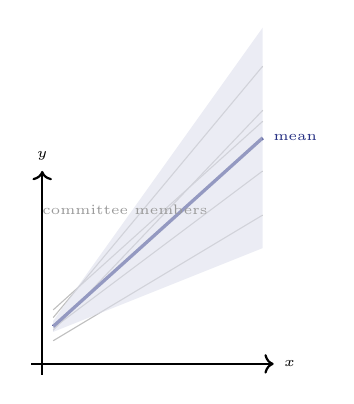
\begin{tikzpicture}[scale=0.7]
        % axes
        \draw[->, thick] (-0.2,0)--(4.2,0) node[right]{\tiny $x$};
        \draw[->, thick] (0,-0.2)--(0,3.5) node[above]{\tiny $y$};
        % committee of lines
        \foreach \s/\i in {0.6/0.3, 0.75/0.5, 0.9/0.8, 1.05/0.4, 1.2/0.6}{
          \draw[gray!50, thin] plot[domain=0.2:4.0] (\x, {\s*\x+\i});
        }
        % mean
        \draw[darkblue, very thick] plot[domain=0.2:4.0] (\x, {0.9*\x+0.5})
          node[right]{\tiny mean};
        % credible band
        \fill[darkblue!15, opacity=0.6]
          plot[domain=0.2:4.0](\x,{0.9*\x+0.5+0.5*\x})--
          plot[domain=4.0:0.2](\x,{0.9*\x+0.5-0.5*\x})--cycle;
        \node[gray!80] at (1.5,2.8) {\tiny committee members};
      \end{tikzpicture}
    \end{column}
  \end{columns}

\end{frame}

% ----------------------------------------------------------------
\begin{frame}{Two Sources of Uncertainty}

  \begin{columns}[T]
    \begin{column}{0.48\textwidth}
      \begin{block}{Aleatoric Uncertainty}
        \textbf{Irreducible} noise inherent in the data-generating process.\\[0.5em]
        \begin{itemize}
          \item Sensor noise, label ambiguity, stochastic environment
          \item \emph{More data does not reduce it}
          \item Also called \textbf{data uncertainty}
        \end{itemize}
        \vspace{0.5em}
        \textbf{Example:} Even a perfect model cannot predict the exact outcome of a coin flip.
      \end{block}
    \end{column}
    \begin{column}{0.48\textwidth}
      \begin{block}{Epistemic Uncertainty}
        \textbf{Reducible} uncertainty due to limited knowledge or data.\\[0.5em]
        \begin{itemize}
          \item Model uncertainty, sparse coverage of input space
          \item \emph{More data CAN reduce it}
          \item Also called \textbf{model uncertainty} or \textbf{knowledge uncertainty}
        \end{itemize}
        \vspace{0.5em}
        \textbf{Example:} A model trained on data from one hospital is uncertain about patients from a different demographic.
      \end{block}
    \end{column}
  \end{columns}

\end{frame}

% ----------------------------------------------------------------
\begin{frame}{Visual Intuition: Aleatoric vs.\ Epistemic}

\begin{center}
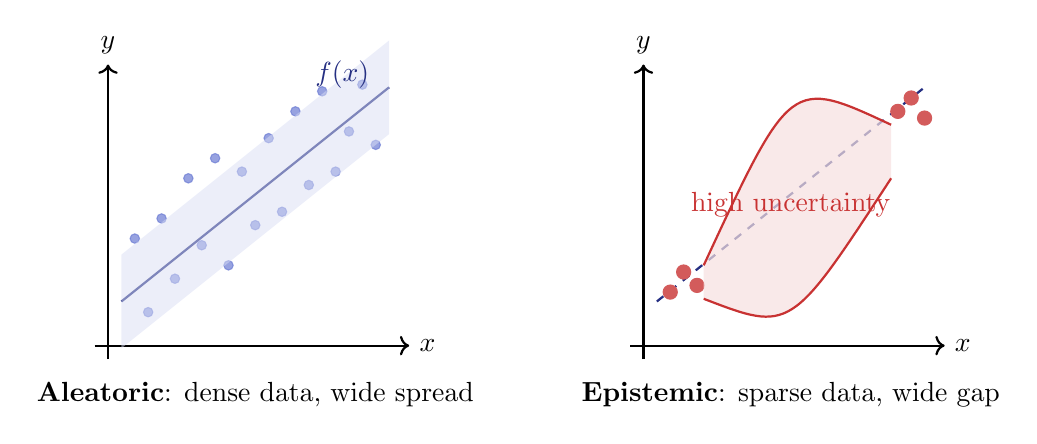
\begin{tikzpicture}[scale=0.85]
  % ---------- LEFT: aleatoric (wide scatter, dense data) ----------
  \begin{scope}[xshift=0cm]
    \draw[->, thick] (-0.2,0) -- (4.5,0) node[right] {$x$};
    \draw[->, thick] (0,-0.2) -- (0,4.2) node[above] {$y$};
    % True function
    \draw[darkblue, thick, domain=0.2:4.2, samples=80]
      plot (\x, {0.8*\x + 0.5});
    % Scattered points (wide noise — aleatoric)
    \foreach \px/\py in {
      0.4/1.6, 0.6/0.5, 0.8/1.9, 1.0/1.0, 1.2/2.5,
      1.4/1.5, 1.6/2.8, 1.8/1.2, 2.0/2.6, 2.2/1.8,
      2.4/3.1, 2.6/2.0, 2.8/3.5, 3.0/2.4, 3.2/3.8,
      3.4/2.6, 3.6/3.2, 3.8/3.9, 4.0/3.0}{
        \filldraw[midblue!80, opacity=0.7] (\px,\py) circle (2pt);
    }
    % Narrow band
    \fill[midblue!20, opacity=0.5]
      plot[domain=0.2:4.2, samples=80] (\x, {0.8*\x + 0.5 + 0.7})
      -- plot[domain=4.2:0.2, samples=80] (\x, {0.8*\x + 0.5 - 0.7})
      -- cycle;
    \node[below] at (2.2, -0.4) {\textbf{Aleatoric}: dense data, wide spread};
    \node[above, darkblue] at (3.5, 3.7) {$f(x)$};
  \end{scope}

  % ---------- RIGHT: epistemic (few points, wide CI in gap) ----------
  \begin{scope}[xshift=8cm]
    \draw[->, thick] (-0.2,0) -- (4.5,0) node[right] {$x$};
    \draw[->, thick] (0,-0.2) -- (0,4.2) node[above] {$y$};
    % True function (hidden from model)
    \draw[darkblue, thick, dashed, domain=0.2:4.2, samples=80]
      plot (\x, {0.8*\x + 0.5});
    % Only a few observed points clustered at the extremes
    \foreach \px/\py in {0.4/0.8, 0.6/1.1, 0.8/0.9, 3.8/3.5, 4.0/3.7, 4.2/3.4}{
      \filldraw[alertred!80] (\px,\py) circle (3pt);
    }
    % Wide epistemic band in the middle
    \fill[alertred!15, opacity=0.7]
      (0.9, 1.2) .. controls (2.2, 4.0) .. (3.7, 3.3)
      -- (3.7, 2.5) .. controls (2.2, 0.2) .. (0.9, 0.7) -- cycle;
    \draw[alertred, thick]
      (0.9, 1.2) .. controls (2.2, 4.0) .. (3.7, 3.3);
    \draw[alertred, thick]
      (0.9, 0.7) .. controls (2.2, 0.2) .. (3.7, 2.5);
    \node[below] at (2.2, -0.4) {\textbf{Epistemic}: sparse data, wide gap};
    \node[alertred] at (2.2, 2.1) {high uncertainty};
  \end{scope}
\end{tikzpicture}
\end{center}
\end{frame}


\begin{frame}{Aleatoric vs. Epistemic}

    \centering
    % Upload an image file named aleatoric-example.(pdf|png|jpg) into the project.
    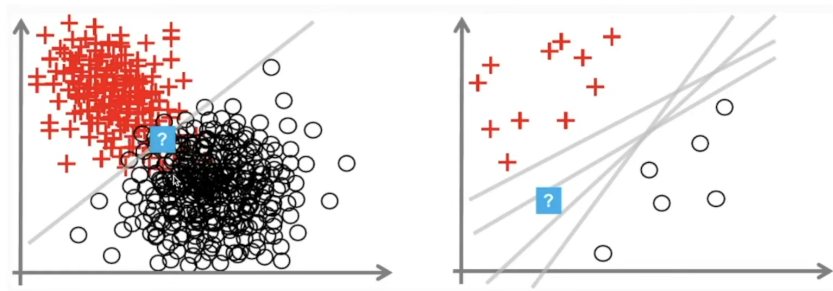
\includegraphics[width=0.8\linewidth]{images/alea_epis.png}
    \vspace{0.2cm}

\end{frame}

% ----------------------------------------------------------------
\begin{frame}{Formal Decomposition of Predictive Uncertainty}

  For a probabilistic model $p_{\btheta}(y \mid x)$ with posterior $p(\btheta \mid \calD)$,
  the \textbf{total predictive uncertainty} decomposes as:

  \begin{alertblock}{Variance Decomposition}
    \[
      \underbrace{\Var_{p(\btheta|\calD)}\!\left[\E[Y\mid x,\btheta]\right]}_{\text{Epistemic}}
      +
      \underbrace{\E_{p(\btheta|\calD)}\!\left[\Var[Y\mid x,\btheta]\right]}_{\text{Aleatoric}}
      =
      \underbrace{\Var[Y\mid x,\calD]}_{\text{Total}}
    \]
  \end{alertblock}

  \begin{itemize}
    \item \textbf{Epistemic term}: Variance of the \emph{conditional mean} across models — how
          much do different plausible parameter settings disagree on the expected output?
    \item \textbf{Aleatoric term}: Expected \emph{residual variance} within each model — noise
          that persists regardless of which model is correct.
  \end{itemize}

  \begin{block}{Why does this decomposition matter?}
    Epistemic uncertainty is \textit{actionable}: collect more data in high-uncertainty regions.\\
    Aleatoric uncertainty is \textit{fundamental}: focus on better labeling or sensor quality.
  \end{block}

\end{frame}

% Slide: Aleatoric vs. Epistemic (image comparison)
\begin{frame}{Epistemic Uncertainty}
  \begin{columns}[T,onlytextwidth]
    \begin{column}{0.48\textwidth}
      \centering
      % Upload an image file named aleatoric-example.(pdf|png|jpg) into the project.
      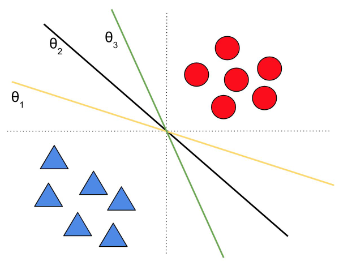
\includegraphics[width=\linewidth]{images/epis2.png}
      \vspace{0.2cm}

    \end{column}
    \begin{column}{0.48\textwidth}
      \centering
      % Upload an image file named epistemic-example.(pdf|png|jpg) into the project.
      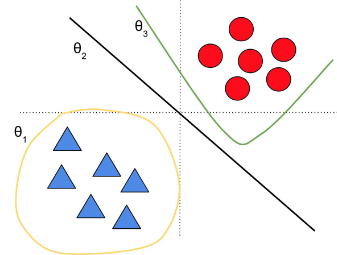
\includegraphics[width=\linewidth]{images/epis3.png}
      \vspace{0.2cm}
    
    \end{column}
  \end{columns}
\end{frame}

\begin{frame}{Epistemic Uncertainty}

    \centering
    % Upload an image file named aleatoric-example.(pdf|png|jpg) into the project.
    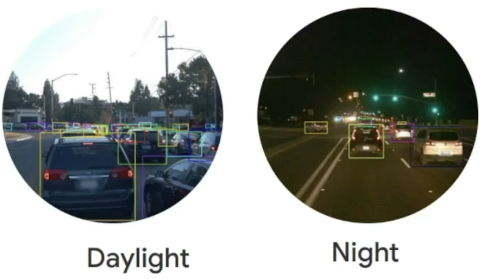
\includegraphics[width=0.8\linewidth]{images/epis_ex.png}
    \vspace{0.2cm}

\end{frame}

\begin{frame}{Aleatoric Uncertainty}

    \centering
    % Upload an image file named aleatoric-example.(pdf|png|jpg) into the project.
    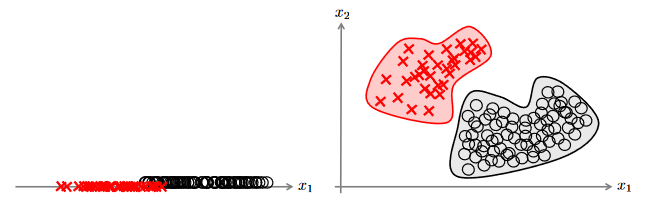
\includegraphics[width=1\linewidth]{images/alea4.png}
    \vspace{0.2cm}

    \scriptsize Battleday et al. 2019 “Improving machine classification using human uncertainty measurements” https://openreview.net/pdf?id=rJl8BhRqF7

\end{frame}

\begin{frame}{Aleatoric Uncertainty}

    \centering
    % Upload an image file named aleatoric-example.(pdf|png|jpg) into the project.
    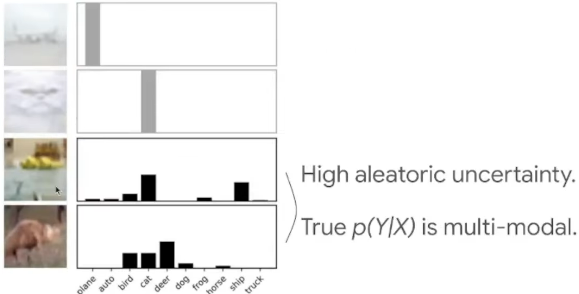
\includegraphics[width=0.8\linewidth]{images/alea.png}
    \vspace{0.2cm}

    \scriptsize Battleday et al. 2019 “Improving machine classification using human uncertainty measurements” https://openreview.net/pdf?id=rJl8BhRqF7

\end{frame}

\begin{frame}{Aleatoric Uncertainty}

    \centering
    % Upload an image file named aleatoric-example.(pdf|png|jpg) into the project.
    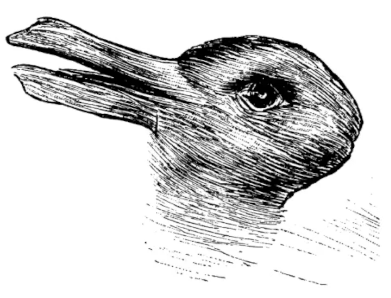
\includegraphics[width=0.5\linewidth]{images/alea3.png}
    \vspace{0.2cm}

    \scriptsize Vaishaal Shankar, Rebecca Roelofs, Horia Mania, Alex Fang, Benjamin Recht, and Ludwig Schmidt. 2020. Evaluating machine accuracy on ImageNet. In Proceedings of the 37th International Conference on Machine Learning (ICML'20), Vol. 119. JMLR.org, Article 801, 8634–8644.

\end{frame}

% =============================================================
\begin{frame}{Practical Guide: Which Uncertainty for Which Task?}

  \begin{center}
  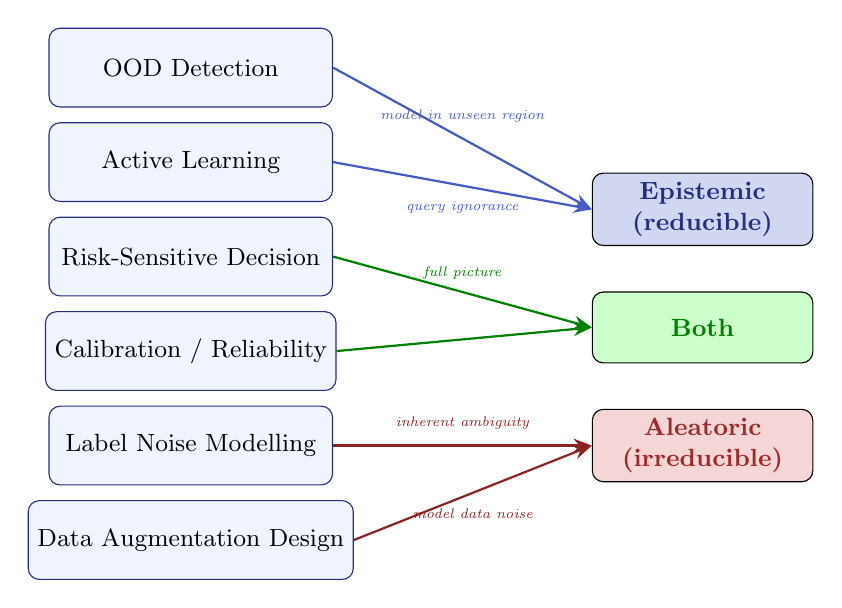
\begin{tikzpicture}[
    box/.style  ={draw=darkblue, rounded corners=4pt, fill=lightblue!20,
                  minimum width=3.6cm, minimum height=1.0cm, align=center, font=\small},
    ubox/.style ={draw, rounded corners=4pt,
                  minimum width=2.8cm, minimum height=0.9cm, align=center, font=\small\bfseries},
    arr/.style  ={-Stealth, thick},
    note/.style ={font=\scriptsize\itshape, align=left}
  ]
    % Tasks
    \node[box] (ood)  at (0, 3.0) {OOD Detection};
    \node[box] (al)   at (0, 1.8) {Active Learning};
    \node[box] (risk) at (0, 0.6) {Risk-Sensitive Decision};
    \node[box] (conf) at (0,-0.6) {Calibration / Reliability};
    \node[box] (lab)  at (0,-1.8) {Label Noise Modelling};
    \node[box] (aug)  at (0,-3.0) {Data Augmentation Design};

    % Uncertainty types
    \node[ubox, fill=midblue!25,   text=darkblue]   (ep) at (6.5,  1.2) {Epistemic\\(reducible)};
    \node[ubox, fill=alertred!20, text=alertred!80!black] (ale) at (6.5, -1.8) {Aleatoric\\(irreducible)};
    \node[ubox, fill=green!20, text=green!50!black] (both) at (6.5, -0.3) {Both};

    % Arrows + short rationale
    \draw[arr, midblue]   (ood.east)  -- (ep.west)   node[note,midway,above=2pt]{\tiny model in unseen region};
    \draw[arr, midblue]   (al.east)   -- (ep.west)   node[note,midway,below=2pt]{\tiny query ignorance};
    \draw[arr, green!50!black] (risk.east) -- (both.west) node[note,midway,above=1pt]{\tiny full picture};
    \draw[arr, green!50!black] (conf.east) -- (both.west);
    \draw[arr, alertred!70!black] (lab.east)  -- (ale.west)  node[note,midway,above=2pt]{\tiny inherent ambiguity};
    \draw[arr, alertred!70!black] (aug.east)  -- (ale.west)  node[note,midway,below=2pt]{\tiny model data noise};

  \end{tikzpicture}
  \end{center}

\end{frame}

\section{Uncertainty Quantification Methods}
% ----------------------------------------------------------------
\begin{frame}{Section Overview}
  \begin{center}
    \Large \textbf{Uncertainty Quantification Methods}\\[1em]
    \normalsize
    \textit{Before we can evaluate uncertainty estimates, we need methods to produce them.\\
    Different methods capture different types of uncertainty — understanding which is which matters.}
  \end{center}
\end{frame}

% ----------------------------------------------------------------
\begin{frame}{Two Types of Uncertainty — A Refresher}

  \begin{columns}[T]
    \begin{column}{0.48\textwidth}
      \begin{block}{Aleatoric Uncertainty}
        \textbf{Irreducible} — inherent randomness in the data.
        \begin{itemize}
          \item Sensor noise, label ambiguity, stochastic processes
          \item Cannot be reduced by collecting more data
          \item Quantified by modelling $p(y \mid x, \btheta)$
        \end{itemize}
        \[
          \Var[y \mid x] = \E_{\btheta}\!\left[\sigma^2(\btheta)\right]
        \]
      \end{block}
    \end{column}
    \begin{column}{0.48\textwidth}
      \begin{block}{Epistemic Uncertainty}
        \textbf{Reducible} — uncertainty about the model/parameters.
        \begin{itemize}
          \item Limited training data, model misspecification
          \item Decreases as more data is observed
          \item Quantified by the spread over $p(\btheta \mid \calD)$
        \end{itemize}
        \[
          \Var_{\btheta \mid \calD}\!\left[\E[y \mid x, \btheta]\right]
        \]
      \end{block}
    \end{column}
  \end{columns}

  \begin{alertblock}{Total Uncertainty = Aleatoric + Epistemic}
    \[
      \underbrace{\Var[y \mid x, \calD]}_{\text{total}}
      = \underbrace{\E_{\btheta}\!\left[\Var[y \mid x, \btheta]\right]}_{\text{aleatoric}}
      + \underbrace{\Var_{\btheta}\!\left[\E[y \mid x, \btheta]\right]}_{\text{epistemic}}
    \]
    (Law of Total Variance — applies to any model with parameter uncertainty)
  \end{alertblock}

\end{frame}

% ----------------------------------------------------------------
\begin{frame}{Methods Overview: What Does Each Capture?}

  \begin{center}
  \renewcommand{\arraystretch}{1.2}
  \begin{tabular}{llcc}
    \toprule
    \textbf{Method} & \textbf{Core Idea} & \textbf{Epistemic} & \textbf{Aleatoric} \\
    \midrule
    Bayesian Neural Networks & Posterior over weights & \checkmark & $\times$ \\
    Deep Ensembles           & Diversity across models & \checkmark & $\times$ \\
    MC Dropout               & Dropout at test time    & \checkmark & $\times$ \\
    Probabilistic Loss Fns   & Output distributional params & $\times$ & \checkmark \\
    Quantile / Interval Loss & Direct interval estimation & $\times$ & \checkmark \\
    Calibration Methods      & Post-hoc rescaling      & \checkmark & \checkmark \\
    Test-Time Augmentation   & Input perturbations     & $\times$ & \checkmark \\
    Conformal Prediction     & Distribution-free coverage & \checkmark & \checkmark \\
    \bottomrule
  \end{tabular}
  \end{center}

  \vspace{0.3em}
  \small \textit{Note: ``captures'' means the method produces a signal correlated with that
  uncertainty type — it does not mean perfect disentanglement.}

\end{frame}


% ----------------------------------------------------------------
\begin{frame}{Bayesian Neural Networks}

  \begin{block}{Core Idea: Place a Prior Over Weights}
    \[
      p(\btheta \mid \calD) \propto p(\calD \mid \btheta)\, p(\btheta)
      \qquad \longrightarrow \qquad
      p(y^* \mid x^*, \calD) = \int p(y^* \mid x^*, \btheta)\, p(\btheta \mid \calD)\, \mathrm{d}\btheta
    \]
  \end{block}

  \textbf{Approximate Inference Options:}
      \begin{itemize}
        \item \textbf{Variational Inference (VI)}: Fit $q_\phi(\btheta) \approx p(\btheta \mid \calD)$
              by minimising KL divergence (e.g.\ \emph{Bayes by Backprop}, Blundell et al.\ 2015)

        \item \textbf{MCMC (HMC/SGLD)}: Asymptotically exact; expensive for large nets
        \item \textbf{MC Dropout}
      \end{itemize}


\end{frame}

% ----------------------------------------------------------------
\begin{frame}{MC Dropout as Approximate Bayesian Inference}

  \begin{block}{Gal \& Ghahramani (2016): Dropout $\approx$ Variational Inference}
    Applying dropout at \textbf{test time} and averaging $T$ forward passes approximates
    integration over a distribution of model weights.
    \[
      \hat{y}^* \approx \frac{1}{T}\sum_{t=1}^T f^{\hat{\btheta}_t}(x^*)
      \qquad
      \hat{\sigma}^2_{\text{epi}} \approx \frac{1}{T}\sum_{t=1}^T \left(f^{\hat\btheta_t}(x^*)\right)^2
      - \left(\hat{y}^*\right)^2
    \]
  \end{block}

  \textbf{Algorithm:}
      \begin{enumerate}
        \item Train with standard dropout (rate $p$)
        \item At test time: keep dropout \textbf{on}
        \item Run $T$ stochastic forward passes
        \item Report mean $\pm$ std as prediction + uncertainty
      \end{enumerate}
      \textbf{Key Hyperparameter:} $T$ (typically 30–100)

\end{frame}

% ----------------------------------------------------------------
\begin{frame}{Deep Ensembles}

  \begin{block}{Lakshminarayanan et al.\ (2017): Train $M$ Models Independently}
    \[
      p(y \mid x, \calD) \approx \frac{1}{M}\sum_{m=1}^M p_{\btheta_m}(y \mid x)
      \quad\longrightarrow\quad
      \hat\mu = \frac{1}{M}\sum_m \mu_m, \quad
      \hat\sigma^2 = \frac{1}{M}\sum_m \!\left(\sigma_m^2 + \mu_m^2\right) - \hat\mu^2
    \]
  \end{block}


  \textbf{Sources of Diversity:}
  \begin{itemize}
    \item Random weight initialisation
    \item Stochastic mini-batch ordering
    \item (Optional) random feature subsampling / dataset bootstrap
  \end{itemize}

  \textbf{Ensemble Predictive Variance Decomposition:}
  \begin{align*}
    \underbrace{\hat\sigma^2_{\text{total}}}_{\text{total}}
    &= \underbrace{\frac{1}{M}\sum_m\sigma_m^2}_{\text{aleatoric}}
      + \underbrace{\frac{1}{M}\sum_m(\mu_m - \hat\mu)^2}_{\text{epistemic}}
  \end{align*}


\end{frame}
\begin{frame}{Proof 1: The Ensemble Mean}

  \textbf{Finding the Mixture Mean ($\hat{\mu}$)} 
  \begin{align*}
    \mathbb{E}[y] &= \int y \left( \frac{1}{M} \sum_{m=1}^M p_m(y \mid x) \right) dy \\[1ex]
    &= \frac{1}{M} \sum_{m=1}^M \int y \, p_m(y \mid x) \, dy \\[1ex]
    &= \frac{1}{M} \sum_{m=1}^M \mu_m 
  \end{align*}

  \begin{block}{Ensemble Mean}
    \[ \hat{\mu} = \frac{1}{M} \sum_{m=1}^M \mu_m \]
  \end{block}
\end{frame}

\begin{frame}{Proof 2: The Total Ensemble Variance}
  \textbf{Finding the Mixture Variance ($\hat{\sigma}^2$)} \\
  We use the standard variance definition: $\text{Var}(y) = \mathbb{E}[y^2] - (\mathbb{E}[y])^2$.
  

  First, find $\mathbb{E}[y^2]$ across the mixture:
  \begin{align*}
    \mathbb{E}[y^2] &= \frac{1}{M} \sum_{m=1}^M \mathbb{E}_m[y^2] 
  \end{align*}
  Since $\text{Var}_m(y) = \sigma_m^2 = \mathbb{E}_m[y^2] - \mu_m^2$, we know $\mathbb{E}_m[y^2] = \sigma_m^2 + \mu_m^2$.
  

  Substitute this and our mean $\hat{\mu}$ back into the variance formula:
  \begin{block}{Total Ensemble Variance}
    \[ \hat{\sigma}^2 = \frac{1}{M} \sum_{m=1}^M (\sigma_m^2 + \mu_m^2) - \hat{\mu}^2 \]
  \end{block}
\end{frame}

\begin{frame}{Proof 3: Variance Decomposition}


  \begin{align*}
    \frac{1}{M}\sum_{m=1}^M (\mu_m - \hat{\mu})^2 
    &= \left(\frac{1}{M}\sum_{m=1}^M \mu_m^2\right) - 2\hat{\mu}\underbrace{\left(\frac{1}{M}\sum_{m=1}^M \mu_m\right)}_{=\hat{\mu}} + \hat{\mu}^2 \\
    &= \left(\frac{1}{M}\sum_{m=1}^M \mu_m^2\right) - \hat{\mu}^2
  \end{align*}

  Substituting this back yields the Law of Total Variance:
  \begin{block}{Final Decomposition}
    \[ \hat{\sigma}^2 = \underbrace{\frac{1}{M}\sum_{m=1}^M\sigma_m^2}_{\text{Aleatoric}} + \underbrace{\frac{1}{M}\sum_{m=1}^M(\mu_m - \hat{\mu})^2}_{\text{Epistemic}} \]
  \end{block}
\end{frame}


% ----------------------------------------------------------------
\begin{frame}{Probabilistic Loss Functions — Aleatoric UQ}

  \textbf{Key idea:} Let the network \emph{predict the parameters} of an output
  distribution.


  \begin{columns}[T]
    \begin{column}{0.48\textwidth}
      \begin{block}{Gaussian NLL Loss (Regression)}
        Model outputs $(\hat\mu(x), \hat\sigma^2(x))$:
        \[
          \calL = \frac{1}{n}\sum_i \left[
            \frac{(y_i - \hat\mu_i)^2}{2\hat\sigma_i^2}
            + \frac{1}{2}\log \hat\sigma_i^2
          \right]
        \]
        \begin{itemize}
          \item $\hat\sigma^2(x)$ models \textbf{input-dependent noise}
          \item Use $\log \hat\sigma^2$ output for numerical stability
        \end{itemize}
      \end{block}
    \end{column}
    \begin{column}{0.48\textwidth}
      \begin{block}{Quantile / Pinball Loss (Regression)}
        Estimate the $\tau$-th conditional quantile $Q_\tau(x)$:
        \[
          \calL_\tau = \frac{1}{n}\sum_i \rho_\tau\!\left(y_i - \hat Q_\tau(x_i)\right)
        \]
        \[
          \rho_\tau(u) = u(\tau - \mathbf{1}[u < 0])
        \]
        \begin{itemize}
          \item Train heads for $\tau \in \{0.05, 0.5, 0.95\}$ to get a PI
          \item No distributional assumption needed
        \end{itemize}
      \end{block}
    \end{column}
  \end{columns}


\end{frame}

% ----------------------------------------------------------------
\begin{frame}{Calibration Methods — Post-Hoc Correction}

  \begin{block}{Motivation}
    A well-trained discriminative model may be \emph{accurate} yet \emph{miscalibrated}
    (often overconfident after softmax). Post-hoc methods correct this on a held-out
    calibration set $\calD_{\text{cal}}$ without re-training.
  \end{block}



  \textbf{Temperature Scaling (Classification):}
  \[
    \hat{p}_k = \text{softmax}\!\left(\frac{\mathbf{z}}{T}\right)_k
  \]
  Scalar $T > 0$ found by minimising NLL on $\calD_{\text{cal}}$;
  $T > 1$ softens (reduces overconfidence).

  \vspace{0.5em}
  \textbf{Platt Scaling:} Fit a logistic regression on top of logits.

  \vspace{0.5em}
  \textbf{Isotonic Regression:}
  Non-parametric monotone mapping from raw probability to calibrated probability.




\end{frame}

\begin{frame}{Test-Time Augmentation (TTA)}

  \begin{block}{Core Idea}
    Generate $T$ augmented versions $\{\tilde x_t\}$ of input $x$ and aggregate
    predictions. Disagreement across augmentations signals uncertainty.
    \[
      \hat p(y \mid x) \approx \frac{1}{T}\sum_{t=1}^T p_{\hat\btheta}(y \mid \tilde x_t),
      \qquad
      \hat\sigma^2_{\text{TTA}} = \frac{1}{T}\sum_t \hat y_t^2 - \bar{\hat y}^2
    \]
  \end{block}


  \textbf{Common Augmentations:}
  \begin{itemize}
    \item \textbf{Images:} flips, crops, colour jitter, Gaussian blur
    \item \textbf{Tabular:} feature masking, additive noise, Bootstrap
    \item \textbf{Text:} synonym replacement, back-translation
    \item \textbf{Time series:} time warping, scaling, jitter
  \end{itemize}


      


\end{frame}

% ================================================================
\section{Evaluating Uncertainty Estimates}
% ================================================================

\begin{frame}{Section Overview}
  \begin{center}
    \Large \textbf{Evaluating Uncertainty Estimates}\\[1em]
    \normalsize
    \textit{A model that says ``I'm not sure'' about everything is perfectly calibrated — and useless.\\
    We need metrics that reward both calibration and sharpness.}
  \end{center}
\end{frame}

% ----------------------------------------------------------------

\begin{frame}{Calibration}
  \begin{itemize}
  
  
   \item \textbf{Meaning:} Calibration measures how well predicted probabilities match observed outcomes, indicating the accuracy of predictive uncertainty.
    \vspace{0.2cm}
    \item \textbf{Interpretation:} A well-calibrated model produces probabilities that reflect true likelihoods. For example, if a model predicts a probability of 0.7 for a positive outcome, that outcome should occur approximately 70\% of the time.
    \vspace{0.2cm}
    \item \textbf{Why it matters:} Calibration helps assess prediction reliability, especially in high-stakes settings where confidence is critical.
    \vspace{0.2cm}

  \end{enumerate}
\end{frame}

\begin{frame}{On Calibration of Modern Neural Networks}
  \begin{columns}[T,onlytextwidth]
    \begin{column}{0.55\textwidth}
      \begin{itemize}
        \item Modern neural networks frequently demonstrate poor calibration compared to their predecessors.
        \item Large models with minimal regularization often struggle to generalize effectively.
        \item Many studies show deep learning can achieve good generalization when measuring discrimination performance.
        \item This suggests high-capacity models are not immune to overfitting; instead, overfitting often appears as probabilistic error rather than straightforward classification error.
      \end{itemize}
    \scriptsize Guo C, Pleiss G, Sun Y, Weinberger KQ. On Calibration of Modern Neural Networks 2017.
    \end{column}
    \begin{column}{0.45\textwidth}
      \centering
      % Upload an image file named calibration-modern.(pdf|png|jpg) into images/.
      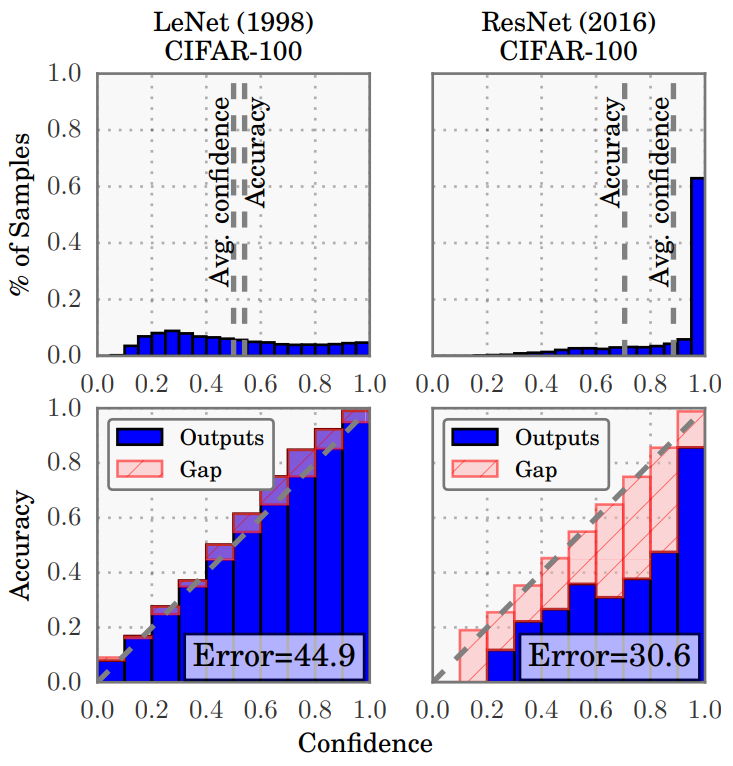
\includegraphics[width=\linewidth]{images/on_cal.png}
    \end{column}
  \end{columns}
\end{frame}

\begin{frame}{Reliability Diagrams and Expected Calibration Error}

  \begin{columns}[T]
    \begin{column}{0.50\textwidth}
      \textbf{Procedure:}
      \begin{enumerate}
        \item Bin predictions by confidence into $M$ equally-spaced bins $B_1, \ldots, B_M$
        \item For each bin, compute:
          \begin{align*}
            \overline{\text{conf}}(B_m) &= \frac{1}{|B_m|}\sum_{i\in B_m}\hat{p}_i \\
            \text{acc}(B_m) &= \frac{1}{|B_m|}\sum_{i\in B_m}\mathbf{1}[\hat{y}_i = y_i]
          \end{align*}
      \end{enumerate}
      \textbf{Expected Calibration Error (ECE):}
      \[
        \text{ECE} = \sum_{m=1}^{M} \frac{|B_m|}{n} \left|\text{acc}(B_m) - \overline{\text{conf}}(B_m)\right|
      \]
      \small Lower ECE = better calibration.\\
      Perfect calibration: ECE $= 0$.
    \end{column}
    \begin{column}{0.47\textwidth}
      \begin{center}
      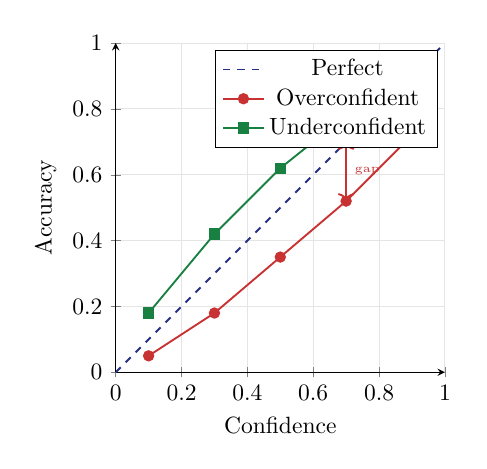
\begin{tikzpicture}[scale=0.85]
        \begin{axis}[
          width=6.5cm, height=6.5cm,
          xlabel={Confidence}, ylabel={Accuracy},
          xmin=0, xmax=1, ymin=0, ymax=1,
          xtick={0,0.2,0.4,0.6,0.8,1.0},
          ytick={0,0.2,0.4,0.6,0.8,1.0},
          grid=major, grid style={gray!20},
          axis lines=left,
        ]
          % Perfect calibration diagonal
          \addplot[darkblue, dashed, thick, domain=0:1] {x};
          \addlegendentry{Perfect}

          % Overconfident model (below diagonal)
          \addplot[alertred, thick, mark=*, mark size=2pt]
            coordinates {(0.1,0.05)(0.3,0.18)(0.5,0.35)(0.7,0.52)(0.9,0.72)};
          \addlegendentry{Overconfident}

          % Underconfident model (above diagonal)
          \addplot[successgreen!80!black, thick, mark=square*, mark size=2pt]
            coordinates {(0.1,0.18)(0.3,0.42)(0.5,0.62)(0.7,0.78)(0.9,0.91)};
          \addlegendentry{Underconfident}

          % Gap annotations
          \draw[alertred, <->, thick] (axis cs:0.7,0.52) -- (axis cs:0.7,0.70)
            node[midway, right, font=\tiny, alertred] {gap};

        \end{axis}
      \end{tikzpicture}
      \end{center}
    \end{column}
  \end{columns}

\end{frame}

\begin{frame}{Brier Score: Intuition and Definition}
  \begin{itemize}
    \item \textbf{Goal:} evaluate probabilistic predictions for classification.
    \item \textbf{Binary case:} for outcome $y \in \{0,1\}$ and predicted probability $p$,
          the Brier score is the squared error $(p-y)^2$.
    \item \textbf{Multiclass case:} with one-hot label $\bm{y}$ and predicted
          probabilities $\bm{p}$,
          \[
            \mathrm{BS} = \frac{1}{N} \sum_{i=1}^N \sum_{k=1}^K (p_{ik} - y_{ik})^2.
          \]
    \item \textbf{Lower is better:} \textbf{measure BOTH discrimination and calibration}.
  \end{itemize}
\end{frame}

\begin{frame}{Proof of Murphy Decomposition (1/3): Setup}
  \textbf{Notation \& Initial Expansion}
  
  \vspace{0.2cm}
  Assume $N$ predictions partitioned into $K$ bins. For bin $k$:
  \begin{itemize}
      \item $n_k$: number of predictions in the bin
      \item $p_k$: predicted probability for items in the bin
      \item $y_{ki} \in \{0,1\}$: $i$-th observed outcome in the bin
      \item $\bar{y}_k = \frac{1}{n_k}\sum_{i=1}^{n_k} y_{ki}$: empirical base rate for the bin
  \end{itemize}

  \vspace{0.2cm}
  The Brier Score (MSE) is:
  \[
    \text{BS} = \frac{1}{N} \sum_{k=1}^K \sum_{i=1}^{n_k} (p_k - y_{ki})^2
  \]

  \vspace{0.1cm}
  Add and subtract the bin base rate ($\bar{y}_k$):
  \[
    \text{BS} = \frac{1}{N} \sum_{k=1}^K \sum_{i=1}^{n_k} \left( (p_k - \bar{y}_k) + (\bar{y}_k - y_{ki}) \right)^2
  \]
\end{frame}

\begin{frame}{Proof of Murphy Decomposition (2/3): Reliability}
  \textbf{Expanding the Square}
  

  Expanding the previous equation yields three terms:
  \begin{align*}
    \text{BS} &= \frac{1}{N} \sum_{k=1}^K \sum_{i=1}^{n_k} \Big[ (p_k - \bar{y}_k)^2 + (\bar{y}_k - y_{ki})^2 \\
    &\quad \quad \quad \quad \quad + 2(p_k - \bar{y}_k)(\bar{y}_k - y_{ki}) \Big]
  \end{align*}


  The cross-term sums to zero because $\sum_{i=1}^{n_k} (\bar{y}_k - y_{ki}) = n_k\bar{y}_k - n_k\bar{y}_k = 0$.

  We are left with \textbf{Reliability} and a term for unexplained variance:
  \[
    \text{BS} = \underbrace{\frac{1}{N} \sum_{k=1}^K n_k (p_k - \bar{y}_k)^2}_{\textbf{Reliability}} \;+\; \underbrace{\frac{1}{N} \sum_{k=1}^K \sum_{i=1}^{n_k} (\bar{y}_k - y_{ki})^2}_{\text{Unexplained Variance}}
  \]
\end{frame}

\begin{frame}{Proof of Murphy Decomposition (3/3): Resolution}
  \textbf{Decomposing the Target Variance}

  Let $\bar{y} = \frac{1}{N}\sum_{k=1}^K n_k \bar{y}_k$ be the global base rate. 
  \begin{align*}
    \text{UNC} &= \bar{y}(1 - \bar{y}) = \frac{1}{N} \sum_{k=1}^K \sum_{i=1}^{n_k} (y_{ki} - \bar{y})^2 \\
    &= \frac{1}{N} \sum_{k=1}^K \sum_{i=1}^{n_k} \left( (y_{ki} - \bar{y}_k) + (\bar{y}_k - \bar{y}) \right)^2 \\
    &= \underbrace{\frac{1}{N} \sum_{k=1}^K \sum_{i=1}^{n_k} (y_{ki} - \bar{y}_k)^2}_{\text{Unexplained Variance}} \;+\; \underbrace{\frac{1}{N} \sum_{k=1}^K n_k (\bar{y}_k - \bar{y})^2}_{\textbf{Resolution}} \;+\; 0
  \end{align*}
  

  Substituting this into the BS equation from Step 2:
  \[
    \text{BS} = \text{Reliability} - \text{Resolution} + \text{Uncertainty} \quad \blacksquare
  \]
\end{frame}
% ----------------------------------------------------------------
\begin{frame}{Brier Score: The Murphy Decomposition}

  As a strictly proper scoring rule, the Brier Score (BS) evaluates both the \textbf{calibration} and \textbf{discrimination} of a probabilistic model by decomposing into three terms:

  \vspace{0.2cm}

  \[
    \text{BS} = \underbrace{\frac{1}{N}\sum_{k=1}^K n_k (p_k - \bar{y}_k)^2}_{\text{Reliability (Calibration)}} 
    \;-\; \underbrace{\frac{1}{N}\sum_{k=1}^K n_k (\bar{y}_k - \bar{y})^2}_{\text{Resolution (Discrimination)}} 
    \;+\; \text{UNC}
  \]

  \vspace{0.3cm}

  \begin{itemize}
      \setlength{\itemsep}{0.5em}
      \item \textbf{Reliability:} How closely the predicted probabilities ($p_k$) match the observed conditional frequencies ($\bar{y}_k$) within $K$ bins. \textit{(Penalty: lower is better)}
      \item \textbf{Resolution:} The model's ability to separate sub-populations with different true event rates from the global base rate ($\bar{y}$). \textit{(Reward: higher is better)}
      \item \textbf{UNC:} The inherent variance of the target variable. It is a property of the dataset, entirely independent of the model.
  \end{itemize}

\end{frame}



% ----------------------------------------------------------------
\begin{frame}{Negative Log-Likelihood (NLL)}

  The \textbf{Negative Log-Likelihood} evaluates the \emph{full predictive distribution} rather than only point accuracy.

  \vspace{0.3cm}

  \begin{block}{Definition}
    For a probabilistic model $p_\theta(y \mid x)$ and dataset $\{(x_i,y_i)\}_{i=1}^n$:
    \[
      \text{NLL} \;=\; -\frac{1}{n}\sum_{i=1}^n \log p_\theta(y_i \mid x_i)
    \]
  \end{block}

  \vspace{0.2cm}

  \begin{itemize}
    \item \textbf{Lower is better:} higher probability mass on true outcomes.
    \item NLL is a measure of \textbf{BOTH calibration and accuracy}

  \end{itemize}

\end{frame}

% ----------------------------------------------------------------
\begin{frame}{Misclassification: Uncertainty Thresholding}
  \begin{columns}[T,onlytextwidth]
    \begin{column}{0.58\textwidth}
      \begin{itemize}
        \item \textbf{Goal:} decide when to \emph{predict} vs. \emph{defer}.
        \vspace{0.2cm}
        \item \textbf{Certainty score (binary):}
        \[
          c(x) = \max\{p(x),\,1-p(x)\}
        \]
        \item \textbf{Decision rule:} predict if $c(x) \ge \tau$; otherwise \textbf{defer}.
        \vspace{0.2cm}
        \item \textbf{Coverage:} fraction of non-deferred samples.
        \item \textbf{Selective accuracy:} accuracy on the covered set.
      \end{itemize}
    \end{column}
    \begin{column}{0.40\textwidth}
      \centering
      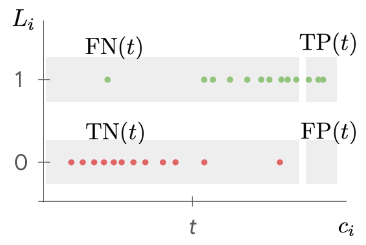
\includegraphics[width=\linewidth]{images/misclass2.png}
      \vspace{0.1cm}
      \scriptsize Higher $\tau$ $\Rightarrow$ fewer predictions, higher confidence.
    \end{column}
  \end{columns}
\end{frame}

\begin{frame}{Misclassification: Confusion Matrix}
  \begin{columns}[T,onlytextwidth]
    \begin{column}{0.56\textwidth}
      \begin{itemize}
        \item \textbf{True Positive (TP):} defer and model would be wrong.
        \item \textbf{False Positive (FP):} defer but model would be correct.
        \item \textbf{True Negative (TN):} predict and model is correct.
        \item \textbf{False Negative (FN):} predict but model is wrong.
      \end{itemize}
      \vspace{0.2cm}
      Since the optimal threshold is often unknown, we can evaluate performance using the area under the curve (AUC), which assesses all possible thresholds.
    \end{column}
    \begin{column}{0.42\textwidth}
      \centering
      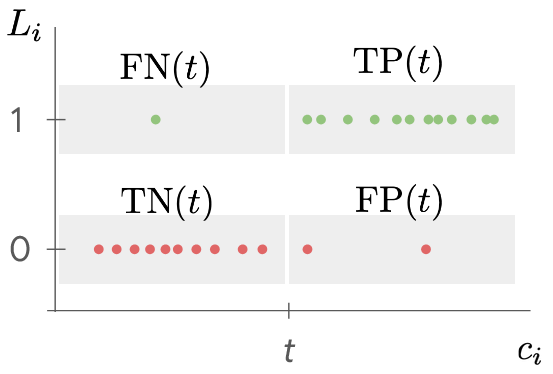
\includegraphics[width=\linewidth]{images/misclass.png}
    \end{column}
  \end{columns}
\end{frame}


\begin{frame}{Interval Coverage and Width for Regression UQ}

  For regression with predictive intervals $[\hat{l}(x), \hat{u}(x)]$:

  \begin{columns}[T]
    \begin{column}{0.50\textwidth}
      \textbf{Coverage (validity):}
      \[
        \text{PICP} = \frac{1}{n}\sum_{i=1}^n \mathbf{1}\!\left[y_i \in [\hat{l}(x_i), \hat{u}(x_i)]\right]
      \]
      Should be $\geq 1-\alpha$ (e.g., 90\%).

      \vspace{0.5em}
      \textbf{Mean Prediction Interval Width (MPIW):}
      \[
        \text{MPIW} = \frac{1}{n}\sum_{i=1}^n \left(\hat{u}(x_i) - \hat{l}(x_i)\right)
      \]
      Should be as \emph{small} as possible given coverage.
    \end{column}
    \begin{column}{0.47\textwidth}
      \begin{center}
      \begin{tikzpicture}[scale=0.80]
        \begin{axis}[
          width=6.5cm, height=5.5cm,
          xlabel={$x$}, ylabel={$y$},
          xmin=0, xmax=6, ymin=-1, ymax=7,
          axis lines=left, grid=major, grid style={gray!20},
          xtick={1,2,3,4,5}, ytick={0,2,4,6},
        ]
          % Predicted mean
          \addplot[darkblue, thick, domain=0.5:5.8, samples=60] {0.8*x + 0.5};
          \addlegendentry{$\hat{f}(x)$}
          % Interval
          \addplot[name path=U, midblue!30, domain=0.5:5.8, samples=60] {0.8*x+1.5};
          \addplot[name path=L, midblue!30, domain=0.5:5.8, samples=60] {0.8*x-0.5};
          \addplot[midblue!25, opacity=0.6] fill between[of=U and L];
          \addlegendentry{90\% interval}
          % Points: inside and outside
          \addplot[only marks, mark=*, mark size=2.5pt, successgreen!70!black]
            coordinates {(1,1.6)(2,2.2)(3,3.1)(4,3.9)(5,4.5)};
          \addplot[only marks, mark=x, mark size=4pt, alertred, very thick]
            coordinates {(1.5,3.5)(4.5,2.0)};
          \addlegendentry{In interval}
          \addlegendentry{Outside interval}
        \end{axis}
      \end{tikzpicture}
      \end{center}
    \end{column}
  \end{columns}

\end{frame}








\begin{frame}{Summary and Takeaways}
  \begin{itemize}
    \item \textbf{UQ focus:} quantify predictive uncertainty to support safe decisions.
    \item \textbf{Key distinctions:} prediction vs.\ confidence vs.\ calibration.
    \item \textbf{Diagnostics:} reliability diagrams, Brier score (Murphy), NLL.
    \item \textbf{Decision tools:} thresholding and coverage--accuracy trade-offs.
    \item \textbf{Regression UQ:} interval coverage (PICP) and width (MPIW).
  \end{itemize}
\end{frame}

\end{document}